\selectlanguage{italian}

L'interazione delle radiazioni con il mezzo in cui si propagano dipende dalla natura delle particelle di cui esse sono composte:
\begin{itemize}
	\item particelle cariche, che hanno un'interazione continua con gli elettroni del mezzo a causa della forza coulombiana:
	\begin{itemize}
		\item particelle cariche pesanti (range tipico $ \sim 10^{-5} \m $);
		\item elettroni veloci (range tipico $ \sim 10^{-3} \m $);
	\end{itemize}
	\item particelle neutre, che invece non subiscono l'interazione coulombiana ma agiscono in maniera discreta, causando un grande scambio energetico per ogni singola interazione (spesso con i nuclei):
	\begin{itemize}
		\item raggi X e $ \gamma $ (range tipico $ 10^{-1} \m $);
		\item neutroni (range tipico $ 10^{-1} \m $).
	\end{itemize}
\end{itemize}
Per quanto riguarda i principali tipi di radiazioni, che rispecchiano ciascuna delle casistiche appena evidenziate:
\begin{enumerate}
	\item raggi $ \alpha $: percorrono qualche centimetro in aria, vengono arrestati da un foglio di carta;
	\item raggi $ \beta $: percorrono qualche metro in aria, vengono arrestati da qualche millimetro di alluminio;
	\item raggi $ \gamma $: a seconda dell'energia, percorrono fino a molte centinaia di metri in aria, vengono arrestati da notevoli spessori di cemento o piombo;
	\item neutroni: la penetrazione dipende dall'energia, vengono arrestati da notevoli spessori di cemento, acqua o paraffina.
\end{enumerate}

\section{Particelle cariche}

Il tipo di interazione dominante tra radiazione e materia sono le collisioni inelastiche con gli elettroni del mezzo: ciò induce vari fenomeni, principalmente l'eccitazione degli atomi, la loro ionizzazione, la fluorescenza e la fosforescenza del materiale (questi ultimi sono causati dal tempo di diseccitazione molto lento degli stati molecolari, ceh genera l'emissione di luce visibile).\\
Dato che le interazioni avvengono principalmente con gli elettroni atomici, si può calcolare il rapporto delle sezioni d'urto coulombiane:
\begin{equation}
	\frac{\sigma_{\text{nucl}}}{\sigma_{\text{atom}}} \sim \frac{\pi R^2}{\pi a_Z^2} \approx \frac{A^{2/3} \cdot 10^{-26} \,\text{cm}^2}{10^{16} \,\text{cm}^2} = A^{2/3} \cdot 10^{-10}
	\label{eq:3.1}
\end{equation}
Il range tipico per questo rapporto è dunque tra $ 10^{-7} $ e $ 10^{-8} $.

\subsection{Scattering e straggling}

A livello cinematico, considerando una particella di massa $ m \gg m_e $ e velocità $ v_0 $ incidente su un elettrone a riposo:
\begin{equation*}
	\begin{cases}
		\frac{1}{2} m v_0^2 = \frac{1}{2} m v_f^2 + \frac{1}{2} m_e v_e^2 \\
		m v_0 = m v_f + m_e v_e
	\end{cases}
	\quad\Rightarrow\quad
	\begin{cases}
		v_f = \frac{m - m_e}{m + m_e} v_0 \\
		v_e = \frac{2m}{m + m_e} v_0
	\end{cases}
\end{equation*}
Dato che $ v_e \approx 2v_0 $, si ha che:
\begin{equation}
	K_e = 4 \frac{m_e}{m} K_0
	\label{eq:3.2}
\end{equation}
Se ad esempio si considera un protone ($ m_p \approx 2000 m_e $), si vede che $ \Delta K_p = \frac{1}{500} K_0 $, quindi in circa 500 collisione esso viene completamente arrestato: questo avviene in pochi micrometri di materiale.\\
Si vede dunque che c'è una perdita di energia nel corso di numerose interazioni: il processo è graduale. Inoltre, al diminuire dell'energia le particelle incidenti tendono a deviare sempre di più dal percorso rettilineo originario a causa degli scattering, andando a creare uno sciame di particelle: questo fenomeno, detto \textit{straggling}, è sia energetico che posizionale, in quanto ci sarà una regione del materiale nel quale è presente la concentrazione più alta di particelle di radiazione.\\
La proiezione della traiettoria di una particella lungo la direzione di propagazione iniziale è detto \textit{range} ed ha un comportamento stocastico: il range sarà distribuito (diffuso) sia posizionalmente (dipendenza dal materiale) che energeticamente (dipendenza dalla particella), infatti si parla di range straggling. Quantitativamente, detto $ d\ve{s} $ il displacement tra uno scattering e l'altro e $ \theta_s $ l'angolo tra $ d\ve{s} $ e la direzione iniziale di propagazione, si definisce il range come:
\begin{equation}
	R(E) \defeq \int ds \braket{\cos \theta_s} = \int_0^E dE \left( \frac{dE}{ds} \right)^{-1} \braket{\cos \theta_s}
	\label{eq:}
\end{equation}
dove $ \frac{dE}{ds} $ è detto \textit{stopping power} ed esprime la perdita di energia per unità di lunghezza percorsa. Si vede subito che il range è più piccolo dell'effettiva traiettoria percorsa: $ \int ds \ge R(E) $.

\subsection{Modello fenomenologico}

È possibile formulare dei modelli fenomenologici per esprimere lo stopping power in funzione delle caratteristiche della particella e del materiale.\\
Un primo modello fu proposto da Lindhardt, che con la sua teoria dell'elettrone descrisse la perdita di energia causata dalla ionizzazione del materiale:
\begin{equation}
	- \frac{1}{\rho} \frac{dE}{ds} \approx \frac{4\pi Z_p^2 e^4}{m_e v^2} Z_t \frac{1}{2} \ln \left[ \frac{2m_e v^2}{I} \right]
	\label{eq:3.4}
\end{equation}
dove $ \rho $ è la densità atomica del materiale, $ Z_t $ il numero atomico degli atomi target, $ Z_p $ quello della particella incidente, $ v $ la sua velocità e $ I $ è la cosiddetta \textit{ionizing energy}, un parametro empirico che rappresenta l'energia d'eccitazione media degli elettroni nel materiale. Si vede che il fattore dominante è il primo, mentre il logaritmo diventa importante per alte velocità.\\
Un modello che descrive meglio le particelle massive ($ m \gg m_e $) anche in regime relativistico è quello dato dall'\textit{equazione di Bethe-Bloch}, che esprime l'average energy loss:
\begin{equation}
	-\frac{1}{\rho} \frac{dE}{ds} \approx 0.1535 \frac{Z_p^2}{\beta^2} \frac{Z_t}{A_t} \left[ 2 \ln \left( \frac{2m_e c^2}{I (1 - \beta^2)} \right) - 2\beta^2 \right] \text{MeV} \text{cm}^2 \text{g}^{-1}
	\label{eq:3.5}
\end{equation}
Empiricamente, si trova:
\begin{equation}
	I = h \braket{\nu_e} =
	\begin{cases}
		(12 Z_t + 7) \ev & Z_t < 13 \\
		(9.76 Z_t + 58.8 Z_t^{-0.19}) \ev & Z_t \ge 13
	\end{cases}
	\label{eq:3.6}
\end{equation}
È importante ricordare gli andamenti dello stopping power in funzione dei vari parametri:
\begin{itemize}
	\item $ \sim \rho Z_t $, maggiore per materiali densi;
	\item $ \sim Z_p^2 $, maggiore per raggi di ioni pesanti;
	\item $ \sim v^{-2} $, maggiore per particelle lente.
\end{itemize}
In particolare, l'andamento $ \sim v^{-2} $ è equivalente a $ \sim K_0^{-1} $: la proporzionalità inversa all'energia della particella incidente è seguita sperimentalmente con buon accordo fino al minimo di ionizzazione del materiale, ovvero all'energia per cui c'è probabilità minore di interazione tra radiazione e mezzo (dunque minore stopping power). Per energie elevate, al limite relativistiche, i termini $ \beta^2 $ diventano dominanti; inoltre, è necessario apportare delle correzioni per considerare le perdite radiative da Bremsstrahlung ed eventuali effetti $ \rho $-dependent nei plasmi.\\
In Fig. \ref{silicon} è possibile osservare come, fissato il mezzo, lo stopping power aumenti come all'aumentare di $ Z_p $ e diminuisca all'aumentare di $ K_0 $; inoltre, si può vedere come gli ioni più pesanti, per raggiungere lo stesso range, necessitino di maggiore energia.

\begin{figure}[!b]
	\centering
	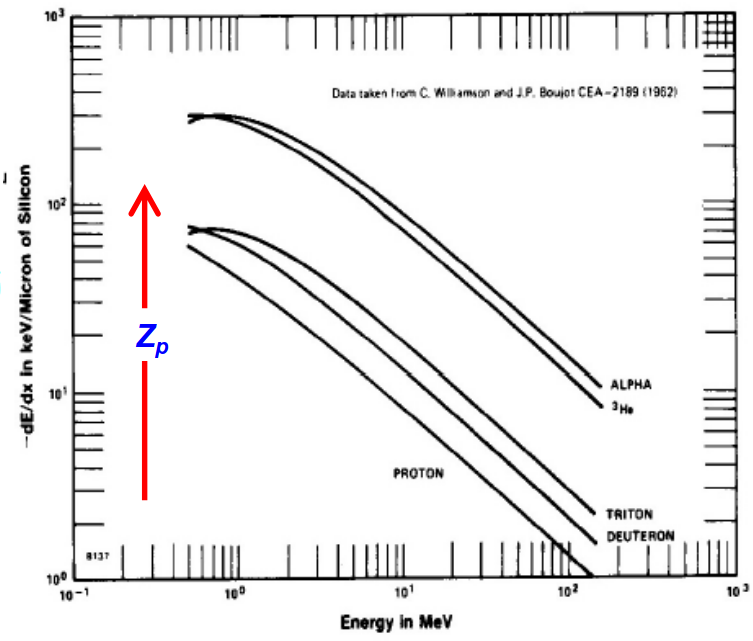
\includegraphics[width=0.45\textwidth]{silicon-sp.png}
	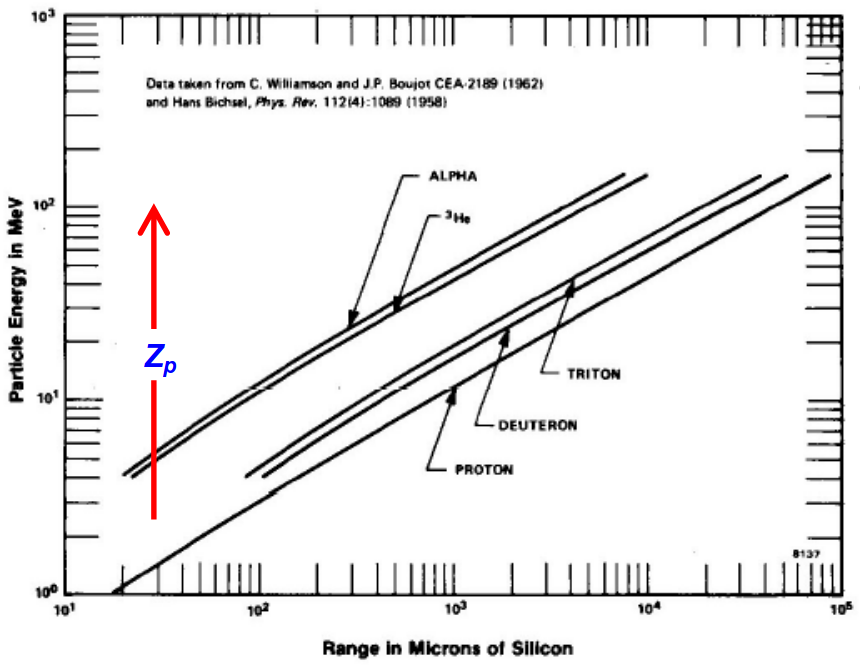
\includegraphics[width=0.495\textwidth]{silicon-r.png}
	\caption{Stopping power and range in Silicon.}
	\label{silicon}
\end{figure}

\paragraph{Particle identification}

Se si ha uno strumento in grado di misurare sia la perdita di energia di una particella carica che la sua energia totale\footnote{Un esempio potrebbe essere un rilevatore al silicio con due strati: uno sottile per misurare la perdita di energia ed uno spesso per fermare la particella, così da poter sommare le due rilevazioni ed ottenere l'energia totale.}, è possibile correlarle ed ottenere dei rami d'iperbole descritti da $ \frac{dE}{ds} E \propto Z_p^2 $. In questo modo si può distinguere tra i vari fasci di particelle ed identificarle, senza però poterne estrarre le masse.

\paragraph{Bragg peak}

La graduale perdita di energia nel range è ciò che sta alla base delle tecniche di adroterapia, ovvero la cura di tumori tramite bombardamento con particelle cariche (soprattutto protoni). Per fare ciò, è necessario conoscere con elevata precisione la perdita di energia specifica (perdita di energia per unità di massa del target) ed il range: quando una particella carica attraversa il corpo umano, essa ionizza tutto il materiale che percorre.\\
Per avere la massima efficacia, sarebbe ideale che la maggior parte dell'energia venisse dissipata in un intervallo specifico del range, così da poter attaccare accuratamente il tumore, ma questo è proprio ciò che avviene: più spazio viene percorso, più la particella perde energia e, di conseguenza, rallenta, quindi la maggior parte dell'energia viene rilasciata alla fine del range, nel cosiddetto \textit{picco di Bragg}. In questo modo, si può regolare il fascio di ioni in modo da far rilasciare la maggior parte dell'energia nel punto in cui si trova la massa tumorale.\\
Per avere un metro di misura della perdita di energia specifica si definisce la dose assorbita $ \frac{dE}{dm} $, misurata in $ \text{gray} \equiv \text{J} / \text{kg} $, dove $ dE $ è l'energia rilasciata nella massa $ dm $ del mezzo dalla radiazione ionizzante. In Fig. \ref{bragg} è possibile vedere come la presenza del picco di Bragg renda i fasci di particelle cariche massive particolarmente efficaci nella cura di tumori.

\begin{figure}[!t]
	\centering
	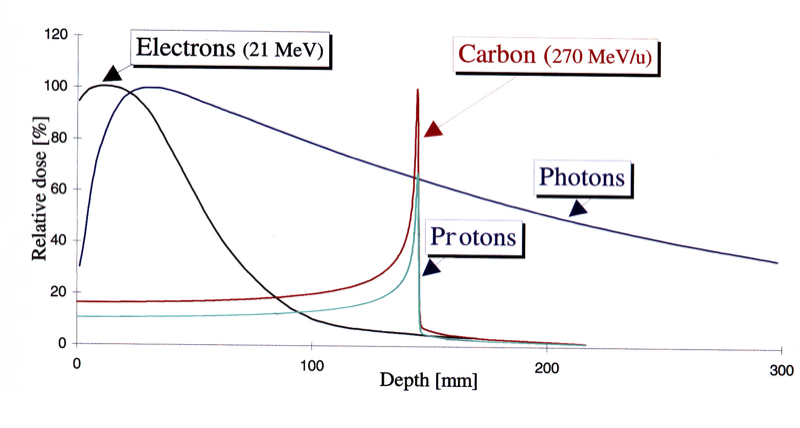
\includegraphics[width=1.00\textwidth]{bragg.png}
	\caption{Absorbed dose for different kinds of radiation.}
	\label{bragg}
\end{figure}

\section{Particelle neutre}

\subsection{Raggi \texorpdfstring{$ \gamma $}{TEXT}}

A differenza delle particelle cariche, i fotoni agiscono in maniera discreta col materiale e la ionizzazioni da essi causati avviene in regioni limitate del mezzo.\\
L'interazione dei fotoni col mezzo può avvenire in tre modi (vedere Fig. \ref{ph-i-p}):
\begin{enumerate}
	\item effetto fotoelettrico, dominante per $ E_{\gamma} < 500 \kev $;
	\item Compton scattering, dominante per $ 500 \kev \le E_{\gamma} \le 2 \mev $;
	\item pair production, dominante per $ E_{\gamma} > 2 \mev $.
\end{enumerate}

\begin{figure}[!b]
	\centering
	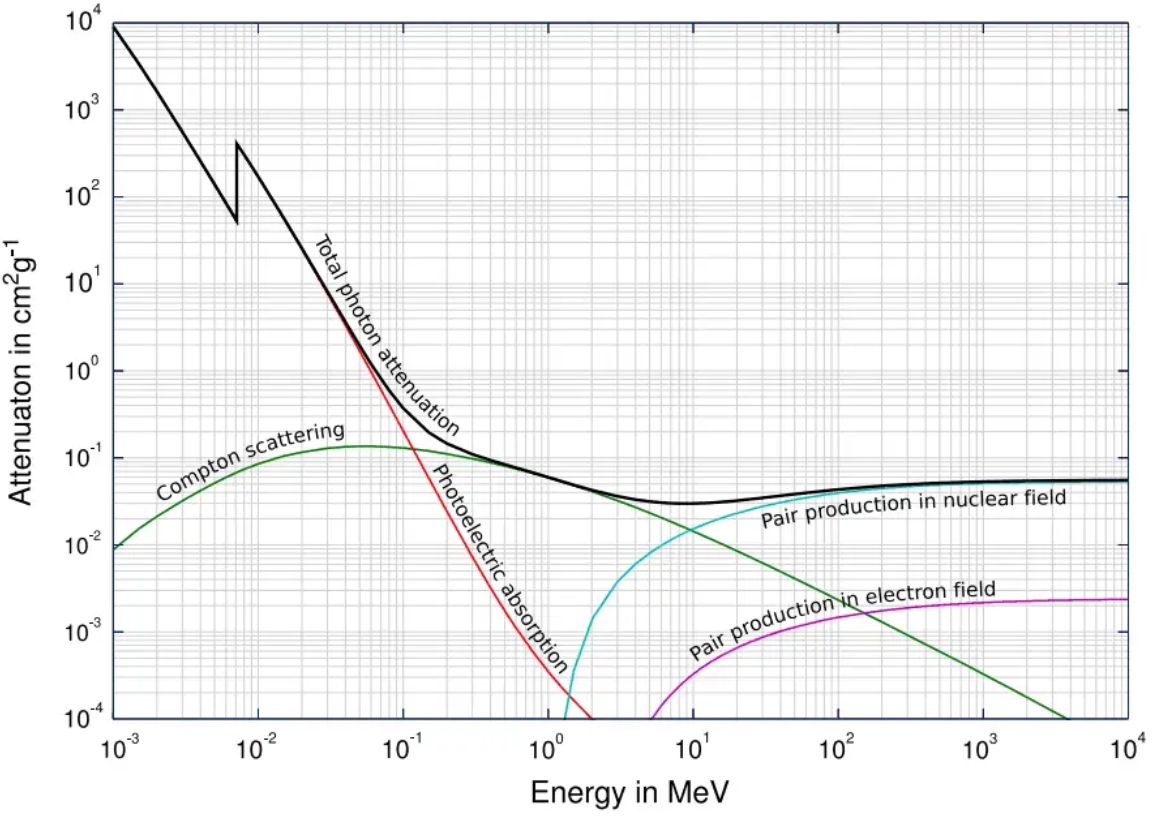
\includegraphics[width=0.70\textwidth]{lin-att-coeff.png}
	\caption{Linear attenuation coefficient for photon interaction.}
	\label{ph-i-p}
\end{figure}

È possibile definire una probabilità d'interazione per unità di lunghezza per ciascuno di questi processi, così da definire il \textit{coefficiente d'attenuazione lineare}:
\begin{equation}
	\mu = \sigma_{\text{ph}} + \sigma_{\text{C}} + \sigma_{\text{pp}}
	\label{eq:3.7}
\end{equation}
In questo modo, si può esplicitare la legge d'attenuazione per l'intensità del fascio di fotoni:
\begin{equation}
	I(x) = I_0 e^{-\mu x}
	\label{eq:3.8}
\end{equation}

\subsubsection{Effetto fotoelettrico}

Avviene quando un raggio $ \gamma $ colpisce un elettrone atomico: il fotone viene completamente assorbito e l'elettrone acquista abbastanza energia per fuoriuscire dall'atomo. In particolare, dato un fotone incidente di pulsazione $ \omega $:
\begin{equation}
	K_e = \hbar \omega - E_n
	\label{eq:3.9}
\end{equation}
dove $ E_n $ è la binding energy dell'elettrone, dipendente dal numero quantico principale e calcolabile con la legge di Moseley:
\begin{equation}
	E_n = Rhc \frac{(Z - \sigma)^2}{n^2}
	\label{eq:3.10}
\end{equation}
con $ Rhc = 13.6 \ev $ costante di Rydberg e $ \sigma $ un parametro dipendente dall'orbitale dell'elettrone (ad esempio $ \sigma_{\text{K}} \approx 3 $ e $ \sigma_{\text{L}} \approx 5 $).\\
Un fenomeno interessante è quello degli \textit{elettroni Auger}. Quando un materiale viene ionizzato, il vuoto creato dall'elettrone espulso viene colmato da un elettrone nella shell successiva: questo salto orbitale comporta l'emissione di un fotone, tipicamente un raggio X, e questa radiazione X è quella che viene tipicamente osservata; può capitare, però, che questo fotone, al posto di essere emesso, venga assorbito da un elettrone in una shell ancora più esterna, il quale viene così emesso dall'atomo: un elettrone di questo tipo viene detto elettrone Auger.

\subsubsection{Compton scattering}

È lo scattering relativistico tra un fotone ed un elettrone. Assumendo l'elettrone inizialmente a riposo:
\begin{equation*}
	\ve{p}_e = \ve{p}_{\gamma} - \ve{p}_{\gamma'} \quad\Rightarrow\quad p_e^2 c^2 = E_{\gamma}^2 + E_{\gamma'}^2 - 2E_{\gamma} E_{\gamma'} \cos \theta
\end{equation*}
dove $ \theta $ è l'angolo tra la direzione incidente e la direzione finale del fotone. Dal bilancio energetico dello scattering $ E_{\gamma} + m_e c^2 = E_{\gamma'} + E_e $ si ottiene:
\begin{equation}
	E_{\gamma'} = \frac{E_{\gamma}}{1 + \frac{E_{\gamma}}{m_e c^2} (1 - \cos \theta)}
	\label{eq:3.11}
\end{equation}
Il fotone con lo scattering subisce anche una variazione di lunghezza d'onda:
\begin{equation}
	\Delta \lambda = \frac{2 \pi}{m_e c} (1 - \cos \theta)
	\label{eq:3.12}
\end{equation}
Dopo un numero di interazioni il fotone viene arrestato: l'ultima interazione è di tipo fotoelettrico.\\
Il Compton scattering è un fenomeno importante quando si costruiscono rilevatori di raggi $ \gamma $: infatti, esso può portare ad una fuoriuscita di fotoni dal rilevatore (se vengono scatterati a determinati angoli), dunque l'energia misurata è parziale e c'è la presenza di un fondo, detto fondo Compton, eliminabile con delle tecniche note.

\subsubsection{Pair production}

È determinata dall'interazione tra un raggio $ \gamma $ ed il campo elettromagnetico presente nel materiale: l'interazione genera due particelle, un elettrone ed un positrone, e l'energia del fotone viene completamente convertita in questa coppia di particelle; successivamente, queste perdono energia all'interno del materiale. In particolare, dato che la massa dell'elettrone/positrone è $ m_ec^2 = 511\kev $, l'energia minima che deve possedere il raggio $ \gamma $ per far avvenire la pair production è $ E_{\text{min}} = 1.022\mev $.\\
Dirac formulò una teoria per spiegare la pair production: il mondo è composto da particelle normali con energia positiva $ E \ge m c^2 > 0 $, mentre esiste il cosiddetto \textit{Fermi sea} composto di particelle con energia negativa $ E \le - m c^2 < 0 $. L'interazione elettromagentica può far transizionare una particella dal Fermi sea al mondo normale, riempiendo il gap energetico di $ \Delta E = 2mc^2 $: il buco lasciato nel Fermi sea è la sua corrispettiva antiparticella.\\
Le prime osservazioni del processo di pair production avvennero nelle camere a bolle: quando un fotone energetico interagisce con un atomo, può avvenire la reazione $ \gamma \rightarrow e^- + e^+ $, eventualmente espellendo anche un ulteriore elettrone dall'atomo. Applicando un campo magnetico è possibile poi studiare il momento e la carica delle particelle così prodotte.

\subsubsection{Interazioni nucleari}

Per raggi $ \gamma $ particolarmente energetici ($ E_{\gamma} \gtrsim 8\mev $) sono possibili anche interazioni a livello nucleare, sebbene meno probabili. Un raggio $ \gamma $ incidente può indurre reazioni all'interno del nucleo, a seguito delle quali possono essere emesse particelle secondarie ad alta energie e/o una sequenza di raggi $ \gamma $ ad energia minore.

\subsection{Neutroni}

A differenza dei fotoni, i neutroni hanno una massa ed è necessario distinguere tra vari range energetici, poiché i processi d'interazione sono molto diversi, sebbene tutti a livello nucleare. Dato che l'interazione nucleare ha un raggio d'azione estremamente ridotto, comparabile al raggio nucleare $ \sim 10^{-15} \m $, i neutroni hanno una bassa probabilità d'interazione: ciò risulta in un minore stopping power ed un maggiore range. Si ricordi inoltre che i neutroni nel nucleo, essendo in stati legati, possono essere stabili, mentre quelli liberi decadono con una vita media di $ 14.76\,\text{min} $.\\
L'interazione con neutroni ha una probabilità che è circa $ 10^{-6} $ volte quella dell'interazione con particelle cariche; in base all'energia (cinetica) $ E_n $ iniziale del neutrone sono possibili diverse interazioni:
\begin{enumerate}
	\item $ E_n \sim 25 \,\text{meV} $: diffusione termica lenta, cattura neutronica (nucleo cattura il neutrone e decade $ \gamma $);
	\item $ E_n < 10 \mev $: scattering elastico (fino alla termalizzazione), cattura neutronica, eccitazione nucleare;
	\item $ E_n > 10 \mev $: scattering elastico ed inelastico, reazioni nucleari (con prodottuzione di particelle cariche secondarie).
\end{enumerate}
I rilevatori di neutroni non rilevano direttamente i neutroni, bensì la radiazione e le particelle secondarie prodotte dai processi nucleari, ad esempio raggi $ \gamma $, particelle cariche ($ p^+ $, $ \alpha $ etc.), altri neutroni, prodotti di fissione e, per neutroni altamente energetici ($ E_n > 150\mev $), prodotti di spallazione: quest'ultimi sono particolarmente pericolosi perché la spallazione pò dar luogo ad uno shower di particelle secondarie estremamente dannose per l'organismo.\\
Come si può vedere in Fig. \ref{n-cross-sec}, fino a $ 10\mev $ la cross-section d'interazione con la materia scala come l'inverso della velocità (ovvero come $ E_n^{-1/2} $), mentre per alte energie sono presenti dei fenomeni di risonanza dovute al fatto che il neutrone può interagire con stati nucleari con funzioni d'onda compatibili.

\begin{figure}[!t]
	\centering
	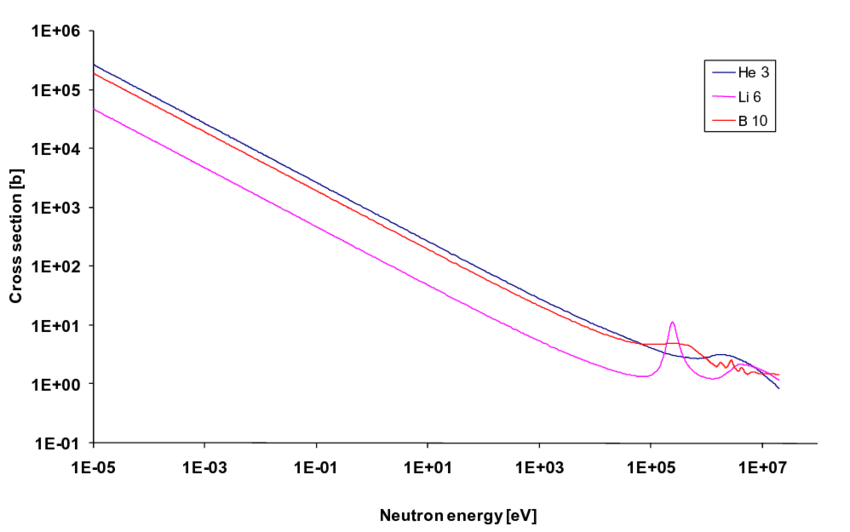
\includegraphics[width=0.60\textwidth]{n-cross-sec.png}
	\caption{Cross-section as a function of neutron energy.}
	\label{n-cross-sec}
\end{figure}

\subsubsection{Neutron detection}

La rilevazione di neutroni avviene tramite la rilevazione diretta delle particelle secondarie prodotte dalle interazioni dei neutroni con la materia. Le cross-sections di tali interazioni sono utili solo per neutroni termici lenti, dunque è necessario un moderatore che, tramite scattering, termalizzi i neutroni: il miglior moderatore è l'idrogeno, poiché con un singolo scattering può assorbire quasi tutta l'energia del neutrone. Infatti, data lo scattering tra un neutrone di energia $ E_n $ ed un nucleo $ ^A_Z\text{X} $, detto $ \theta $ l'angolo tra la direzione incidente e la direzione risultante del neutrone, si ha che:
\begin{equation*}
	E_n' = E_n \left[ 1 - \frac{2 m_n M_A}{(m_n + M_A)^2} (1 - \cos \theta) \right] \approx E_n \frac{A^2 + 2A \cos \theta + 1}{(A + 1)^2} \quad\Rightarrow\quad \left( \frac{A - 1}{A + 1} \right)^2 E_n \le E_n' \le E_n
\end{equation*}
Si trova dunque che l'average energy loss è in percentuale pari a:
\begin{equation}
	\bigg\langle \frac{\Delta E_n}{E_n} \bigg\rangle = \frac{2A}{(A + 1)^2}
	\label{eq:3.13}
\end{equation}
che è massima per $ A = 1 $.\\
Per quanto riguarda i neutroni lenti ($ E_n < 0.5 \ev $), lo scattering elastico non favorisce la rilevazione, poiché l'energia ceduta al nucleo è poca per essere rilevata. Sono invece preferibili le reazioni nucleari neutron-induced, le quali producono particelle secondarie ($ \gamma $, $ p^+ $, $ \alpha $ etc.) abbstanza energetiche da essere rilevate.










